\section{Experiments}
\label{sec:eval}

In this section, we first evaluate the quality of our inferred schemas,
then we perform experiments on the task of link prediction and triple classification.
Finally, we discuss and analyze the errors in our system.

\subsection{Experimental Setup}

\textbf{Knowledge bases.}
We use two knowledge bases throughout our experiments: {\bf FB3m} and {\bf FB15k}.
%We use three knowledge bases throughout our experiments:
%FB15k, FB15k-type and FB (full version).
%FB15k \cite{bordes2013translating} is a widely used benchmark dataset in the task of link prediction and triple classification.
FB15k~\cite{bordes2013translating} is a subset of Freebase 
containing 14,951 entities, 1345 predicates, and 483,142 triple facts.
%Triples in FB15k are split into training / validation / testing parts.
%In order to keep a fair comparison,
We use triples from training split as our knowledge base.
%since all evaluating triples come from OpenIE system.
%Note that FB15k doesn't contain IsA relationship, thus we construct
%a new knowledge base called FB15k-type by adding type information
%of all entities into FB15k.
%Besides, we use Freebase dump of June 2015~\cite{freebase:datadumps}
%as the full version of FB.
%We use these two complementary knowledge bases in link prediction task.
%\tabref{tab:fb-size} shows the statistics of these KBs.
Besides, we construct FB3m from the Freebase dump released of June 2015~\cite{freebase:datadumps},
which contains 3 million popular entities and 50 million triple facts (100 times larger than FB15k).
%Compared with the full dump, FB3m is light-weighted but still
%contains the most valuable knowledge.

\noindent
\textbf{Relation datasets.}
We construct three relation datasets for experiments.
The first two datasets, called ``\textbf{PATTY-100}'' and ``\textbf{PATTY$^+$-100}'',
are extracted from PATTY \cite{nakashole2012patty} OpenIE system, each containing
100 natural language relations.
%We select PATTY \cite{nakashole2012patty} as the OpenIE dataset.
%called ``PATTY-100''.
PATTY contains more than 200,000 different natural language relation synsets
with millions of entity pairs extracted from Wikipedia.
Each entity in PATTY is linked to Freebase through a unique Wikipedia page.
PATTY-100 is for experiments related to FB15k, and contains relations with high
support in PATTY such that all the entities can be found in FB15k.
Conversely, PATTY$^+$-100 is for FB3m related experiments.
It is sampled from all of PATTY and may contain more complex and long-tail relations.
On average, each PATTY-100 relation has a support of 180 facts in
FB15k, and each PATTY$^+$-100 relation has a support of 388 facts in FB3m.
%From top 1,000 distinct PATTY relations sorted by the number of
%relation instances where both arguments are linked to FB15k,
%we randomly pick 100 relations for evaluation. %, called ``PATTY-100''.
%On average, each relation in PATTY-100 contains 180 instances linked to FB15k,
Both PATTY datasets are split into training / validation / testing sets (64\% : 16\% : 20\%).
The third dataset, called ``\textbf{FB15k-37}'', consists of 37 popular predicates
in the domains of ``people'', ``location'' and ``sports'', sampled from FB15k.
FB15k-37 is a subset of FB122 \cite{guo2016jointly},
removing predicates with too small testing data,
and each predicate has at least 10 testing triples.
Experiments on FB15k-37 treats our system as a classic KBC system.

%From top 1,000 distinct PATTY relations sorted by the number of
%relation instances, we randomly pick 100 relations for evaluation.
%Each relation contains 180 instances on average, and we split them into
%training / validation / testing sets (64\% : 16\% : 20\%).
%By manual inspecting, 18 relations are considered complex relations,
%and while the remaining relations are classified as ``ordinary'' relations.

%\begin{table}[ht]
%	\small
%	\centering
%	\caption{Statistics of Freebase used in experiments. \KQ{to be updated.}}
%	\begin{tabular}{|c|c|c|c|}
%		%\toprule
%		\hline
%		Dataset				&	FB15k	&	FB15k-type	&	 FB		\\
%        \hline
%		%Ordinary entities	& 50,718,028	& 3,000,000		&		\\
%        %\hline
%        %Mediator entities	& 36,131,437	& 7,301,261		&		\\
%		%\hline
%		Total entities		&	14,951	&	14,951	&	86,849,465	 \\
%		\hline
%		Distinct relations	&	1,345	&	1,345	&	4,932	\\
%        \hline
%		Types 				&	0		&	xxxx	&	2,071	\\
%		\hline
%		IsA relationships	&	0		&	yyyy	&	zzzz	\\
%		\hline
%		Triple facts		&	483,142	&	483,142	& 280,788,583	\\
%		\hline
%	\end{tabular}%
%	\label{tab:fb-size}%
%\end{table}

\noindent
\textbf{State-of-the-art comparisons.}
For embedding techniques, we take TransE \cite{bordes2013translating},
KALE \cite{guo2016jointly}, TEKE \cite{wang2016text} and
HOLE \cite{nickel2015holographic} as our comparisons.
%TransE models the confidence of a triple fact as vector translations on the
%embeddings of the predicate and two entity arguments.
%%TransE models a relationship as operating translations on the embeddings of
%%subject and object entities. \KQ{Change all subject, object into head, tail??}
%KALE and TEKE are two extensions of TransE.
%KALE introduces logical rules as the combination of atom triple facts with logical connectives,
%therefore the model can learn embeddings from both positive triples and rules.
%TEKE enables each relation to own different representations for different subject and object
%entities, by leveraging the rich context information of a triple fact from web text corpus.
%HOLE is a novel compositional embedding model for representing relationships,
%which is based on the circular correlation of entity vectors.
%
For rule induction techniques, we compare with two models:
SFE \cite{gardner2015efficient} and AMIE+ \cite{galarraga2015fast}.
%One traditional model, called Path Ranking Algorithm \cite{lao2011random},
%extracts all possible paths connecting subject and object entities,
%then learns a feature-based model to represent each relation,
%and SFE is an extension of PRA model, by adding extra subgraph features
%from the surrounding of subject and object entities in the knowledge base.
%AMIE+ first searches possible structures, and then calculates the confidence score
%of each structure by a simple counting strategy in positive triple facts
%(without the step of weight learning).
We also considered Coupled PRA model \cite{wang2016knowledge}
as a comparison. However,
because different relations share almost no entity
pairs in PATTY-100,
the model would degenerate into the traditional PRA model
and hence be strictly superseded by SFE.

\noindent
\textbf{Implementation details.}
We evaluate two variants of our approach: Ours-SC (producing schemas with constraints)
and Ours-SK (schemas skeleton only) .
%The only difference between them is whether
%to explore constraints in schema generation (\secref{sec:candgen}).
%Ours-SK only picks skeletons as candidates (without searching for constraints),
%while Ours-SC is allowed to use all candidate schemas.
%We evaluate our approach under several settings.
%In candidate generation step, we compare two settings:
%``use-skeleton-only'' and ``use-whole-schema'', based on
%whether to explore constraints.
%The first specification only extract path candidates without generating
%constraints, while the latter one is free to use all candidate schemas.
%In schema inference step, we compare two strategies ``random walk''
%and ``zero-one'', described in \secref{sec:schema}.
%\KQ{Will update approach part, mentioning these notations.}
For both variants,
%For each specification, we select the size of priority queue in
%in order to observe how the result varies with the number of candidate schemas.
we set the maximum skeleton length $\tau = 3$,
\footnote{
%Our approach works regardless of the skeleton length. However,
We observed that $\tau > 3$ costs significantly more time with no
substantial benefits.}
%$\tau = 3$,
%tune the minimum support ratio $\gamma$ as in \{5\%, 10\%, 15\%, 20\%\},
%the smoothing parameter $\alpha$ in \{1e-6, 1e-5, 1e-4\}
%and the size of priority queue in
%\{1000, 2000, 3000, 4000, 5000\}.
%||||||| .r20267
%$\tau = 3$,
%tune the minimum support $\gamma$ as in \{5\%, 10\%, 15\%, 20\%\},
%the smoothing parameter $\alpha$ in \{1e-6, 1e-5, 1e-4\}
%and the size of priority queue in
%\{1000, 2000, 3000, 4000, 5000\}.
the size of the priority queue to be 5000.
We tune the minimum support $\gamma$ in the range of \{5\%, 10\%, 15\%, 20\%\},
the smoothing parameter $\alpha$ in \{1e-6, 1e-5, 1e-4\}
and the learning rate in \{0.02, 0.05, 0.1\} on the validation set.
%\KZ{Shall we also eval the effect of different $\tau$? To justify
%why 3 is the right choice.}
%\KQ{Added a footnote here.}
For comparison, we use the existing code for
AMIE+ \footnote{https://www.mpi-inf.mpg.de/departments/databases-and-information-systems/research/yago-naga/amie/},
and SFE system provided by Gardner et al.~\shortcite{gardner2015efficient}
\footnote{https://github.com/matt-gardner/pra},
KALE system by Guo et al.~\shortcite{guo2016jointly},
HOLE and TransE by Nickel et al.~\shortcite{nickel2015holographic}
\footnote{https://github.com/mnick/scikit-kge},
and implement TEKE system by ourselves based on TransE.
All the embedding systems adopt the max-margin model during the learning step.
For KALE, we tune the learning rate in \{0.02, 0.05, 0.1\} and the margin
in \{0.1, 0.12, 0.15, 0.2\}.
For TransE, TEKE and HOLE, we tune the learning rate in \{0.05, 0.1, 0.2\} and the margin
in \{0.5, 1.0, 1.5, 2.0, 2.5\}.


%TODO: Add detail about the other state-of-the-arts.

\subsection{Schema Quality Evaluation}

In this experiment, we focus on how the explicit semantic structure bridges
the gap between Freebase and PATTY$^+$-100 relations.
We compare the top schemas (a.k.a. rules)
of 4 selected example relations produced by Ours-SC, Ours-SK, AMIE+ and SFE,
all of which considered rule induction methods.
The experiment is performed on FB3m, so that each model
can find more different structures.
For each relation from PATTY$^+$-100, we rank the
candidate schemas from Ours-SC and Ours-SK by the learned probability distribution,
while SFE ranks the path features by their feature weights,
and AMIE+ ranks all the rules by their confidence score,
which is the precision of the rule over triple facts in training data.
%Due to many specific rules with the same and highest confidence = $1.0$ in AMIE+,
%we manually pick the most appropriate rule from them.

\figref{fig:relation-example} shows the comparison.
We can learn from examples that:
1) The constraint edges help create more precise semantics.
   Compared with Ours-SK, the schema-based approach learns almost the perfect
   schemas on each example.
2) The quality of top structures from AMIE+ and SFE is not as good as our results.
   AMIE+ ranks rules by confidence and hence prefers more specific rules.
   Once the search depth is increased to 4 or more, the system
   uses huge amount of memory and doesn't return.
   %That's because AMIE+ lacks a tradeoff step, thus top rules always have a high precision
   %but low recall.
   %, therefore we could find rules with necessary constraints  .ranking by confid
   In SFE, the wildcard edge brings about a large amount of flexible path features,
   but most of them don't have clear semantics, and hard to construe by human.


\begin{figure*}[t]
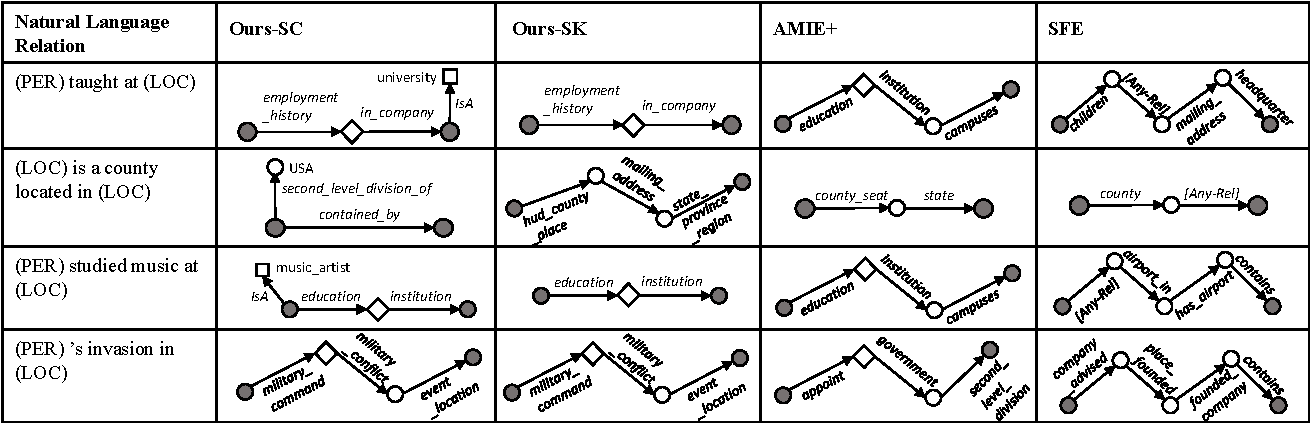
\epsfig{file=case-crop.eps, width=2\columnwidth}
\centering
\caption{Top schemas produced by four systems on 4 complex relations.
%We list top-3 schemas along with probabilities for each relation.
Circle node indicates entities or variables, the two black circles represents
$x_{subj}$ and $x_{obj}$ respectively. Square node represents a type
and diamond node represents a mediator (an n-ary predicate).}
\label{fig:relation-example}
\end{figure*}



As a complementary evaluation, we perform a human judge experiment
on the quality of top ranked schemas produced by Ours-SC and Ours-SK.
%3 annotators, who are familiar with Freebase structure,
%are required to label top 5 schemas of each relation
The evaluators are 3 non-author annotators who are familiar with Freebase.
For each relation, up to top 5 schemas with a probability larger than 0.05 is
labeled with a score in \{0, 0.5, 1\},
indicating ``irrelevant schema'' (semantic drift on the skeleton),
``partial match'' (the skeleton makes sense, but constraints can be improved) and
``perfect match'' (both skeleton and constraints are suitable), respectively.
We first compute the average score for the top $n$ schemas per relation and annotator,
then average these scores over all relations and all annotators to produce
AvgSc@$n$.
The inter-annotator agreement is 0.541 by Kappa coefficient.
As shown in \tabref{tab:average-score}, the schema-based approach
improves the result by up to 13\%.

\begin{table}[t]
	\small
	\centering
	\caption{AvgSc@$n$ results on top-ranked schemas.}
	\label{tab:average-score}
	\begin{tabular}{c|ccc}
						&	n=1		&	n=3		&	n=5			\\
		\hline
		Ours-SK			&	0.44	&	0.37	&	0.34		\\
		Ours-SC			&	\textbf{0.47}	&	\textbf{0.40}	&	\textbf{0.38}
	\end{tabular}
\end{table}


\subsection{Link Prediction}
This task is to predict the missing object in the triple ($e_{subj}$, $r$, $?$),
or the missing subject in ($?$, $r$, $e_{obj}$).
Following the evaluation protocol of KALE \cite{guo2016jointly},
for each triple ($e_{subj}$, $r$, $e_{obj}$) in testing set,
we replace $e_{obj}$ by any other entities $e'_{obj}$ in the knowledge base,
forming a list of wrong triples ($e_{subj}$, $r$, $e'_{obj}$), with only one
positive triple in it.
By using \eqnref{eqn:score-def}, we calculate the score of each prediction in the list
and rank them in descending order,
returning the rank of the correct $e_{obj}$ among all other wrong entities.
Similarly, we can get the rank of $e_{subj}$ at the subject side.
To be consistent with the state-of-the-art systems, we aggregate over all testing triples,
reporting the mean reciprocal rank (MRR)
%, the median value of the ranks (MED),
and the proportion of ranks no larger than $n$ (Hits@$n$, or H@$n$ for short).
%Note that a \textit{lower} MED value indicates a better model.
For each setting, we tune all the parameters based on the MRR score on the validation set.
%\KZ{What about macro F1?}
%\KQ{Nothing to do with F1 in link prediction task, it's in triple classification.
%However, we didn't get a perfect win in F1 metrics, and other papers didn't report F1 also.
%So didn't we.}

Due to the existence of one-to-many relations, some wrong triples ($e_{subj}$, $r$, $e'_{obj}$)
are actually correct and already observed
in the dataset (either in training, validation or testing).
In this case, we follow TransE \cite{bordes2013translating}
and create two settings called ``raw'' and ``filtered''.
In the filtered setting, we remove such correct triples from the triple list
before calculating the rank of each prediction.
Conversely, in the raw setting, we don't remove any triples.


%
%We perform the evaluation on FB15k under filtered setting \KZ{What is this
%setting? Never mentioned before?}.
%\figref{fig:trend-with-budget} shows how the MRR results
%\KQ{on validation set}, vary with the number of candidate schemas.
%From the results, we observe that:
%1) The MRR result increases with the number of candidate schemas in
%every setting, which indicates that larger number of candidates
%leads to a better model.
%2) Compare with strategies on candidate generation, use-whole-schema
%outperforms use-skeleton-only, demonstrating the capability of constraints
%to represent natural language relations.
%3) \KQ{random walk v.s. zero-one, need to get real results before the analysis.}
%
%%\KQ{Figure to be plotted: budget 1k~5k  *  4 different specifications.}
%\begin{figure}[th]
%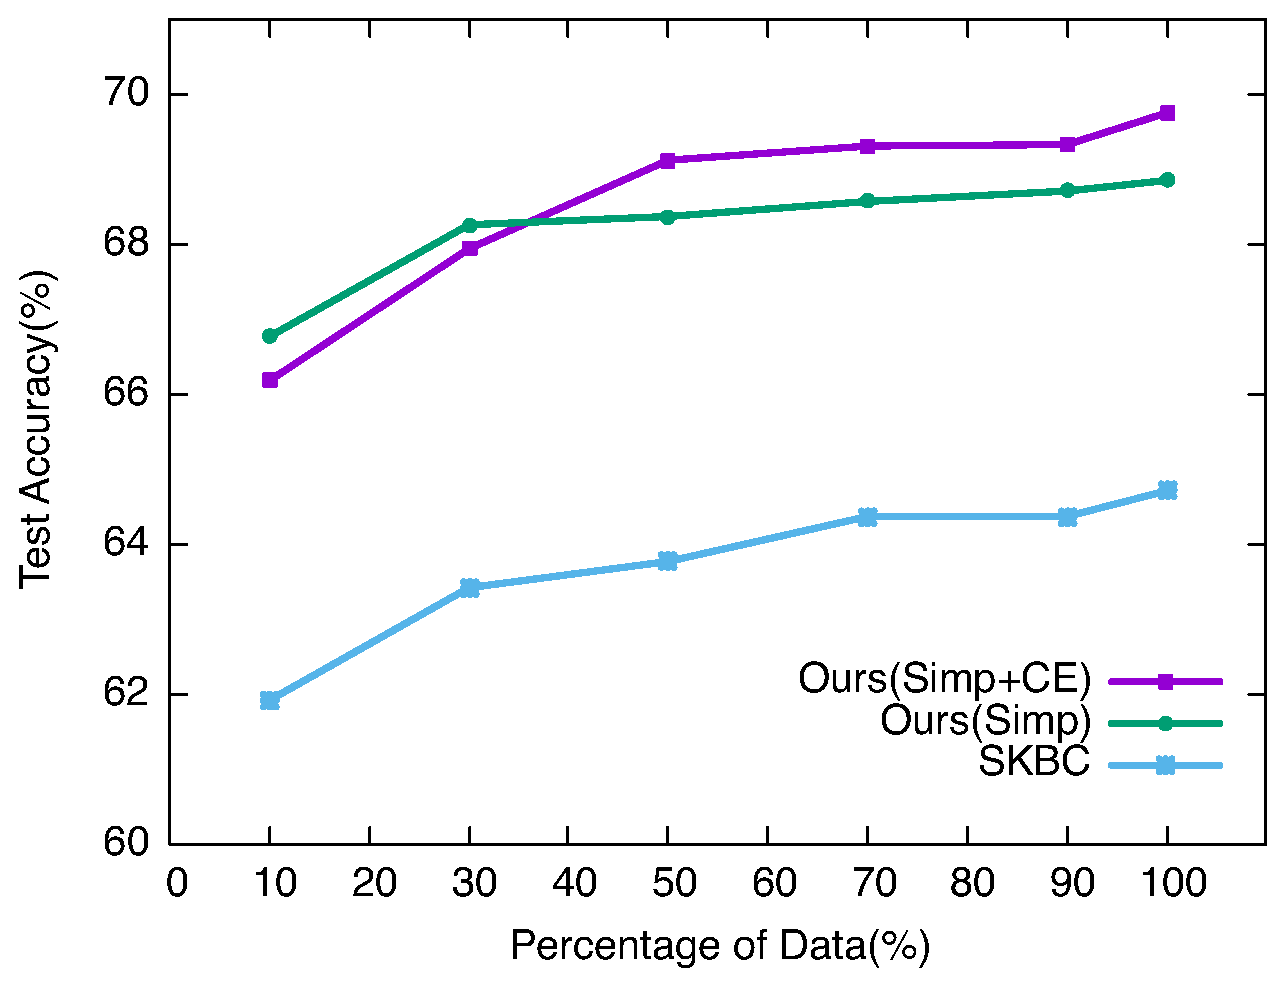
\epsfig{file=trend.eps, width=0.65\columnwidth}
%\centering
%\caption{
%	The trend of link prediction results on FB15k (filtered setting).
%	X axis: size of priority queue,
%	Y axis: MRR score. \KQ{content to be updated.}
%}
%\label{fig:trend-with-budget}
%\end{figure}

%We first evaluate our approach and state-of-the-art systems on PATTY-100 relations.
%Then we compare our approach with state-of-the-art models.
%\KQ{Need to say a little bit about the parameters we used here.}
%\tabref{tab:link-pred-patty} %and \tabref{tab:link-pred-filtered}
%shows the link prediction results on FB15k.

%\KZ{Due to memory issues of the code, SFE method failed to produce any result.
%This is a bit strange: you pick SFE as a comparison but it doesn't work for
%link prediction at all! Better fix this!}
%As we can see, our approach outperforms both embedding and
%other rule induction models.



We perform link predication on FB15k in order to compare with embedding models.
In the following experiments, we use $\gamma=10\%$, $\alpha=1e-4$ and learning rate = 0.1
as the best parameters to achieve the highest filtered MRR score
on the validation set of PATTY-100.
\tabref{tab:link-pred-patty} and \tabref{tab:link-pred-fb15k} shows
the results for PATTY-100 and FB15k-37 respectively.
SFE ran out of memory for both data sets because it needs to enumerate all
possible entities in the KB, and hence is excluded from the tables.
For PATTY-100 relations, our schema based approach outperforms
both embedding and other rule induction models.
Meanwhile, for FB15k-37 predicates, Ours-SK shows nearly the same performance as Ours-SC.
That's because predicates in FB15k-37 may have an equivalent form in KB,
for example, $location.location.containedby \rightarrow !location.location.contains$,
where ``$!$'' indicates the reverse of a predicate, therefore skeletons are precise
enough to represent such predicates.
Furthermore, link predication results on natural language relations are relatively lower
than those on KB predicates.
%Comparing the results on different set of relations,
%the improvements on complex relations are much more significant than those
%on ordinary relations, indicating the usefulness of the extra constraints
%in representing complex relations.
%Besides, the link prediction results on natural language relations
%are relatively lower than
%those results evaluated on FB15k relations \cite{guo2016jointly}.
Two possible reasons are:
1) Each predicate in FB15k-37 has up to thousands of supported instances in FB15k,
while a natural language relation from PATTY-100 only has about 115 training instances.
2) Natural language relations are semantically more ambiguous than KB predicates,
therefore triple facts of different semantics may be mixed during information extraction.
On the other hand, knowledge bases are carefully curated and contain less ambiguity.

\begin{table}[b]
	\small
	\centering
	\caption{Link prediction results on PATTY-100 relations.}
	\label{tab:link-pred-patty}
	\begin{tabular}{|c|ccc|ccc|}
		\hline
				&	\multicolumn{3}{c|}{Raw}
				&	\multicolumn{3}{c|}{Filtered}	\\
		\cline{2-7}	
				&	MRR	&	H@3	&	H@10
				&	MRR	&	H@3	&	H@10		\\
		\hline
		TransE
				&	0.112	&	12.4	&	27.1
				&	0.129	&	14.5	&	29.9	\\	%m1.75_lr0.10
		KALE
				&	0.112	&	12.5	&	25.4
				&	0.125	&	14.4	&	27.5	\\	%Test-base-k100-d0.15-ge0.02-gr10-filt.eval_KQ
		TEKE
				&	0.101	&	10.9	&	24.1
				&	0.114	&	12.6	&	26.3	\\
		HOLE
				&	0.109	&	10.5	&	23.3
				&	0.121	& 	12.3	&	25.8	\\	%log.hole_d100_m0.25_lr0.05
		%AMIE+
		%		&	0.119	&	23.5
		%		&	0.132	&	24.4	\\
		AMIE+
				&	0.148	&	16.5	&	29.3
				&	0.174	&	19.5	&	\textbf{31.9}	\\
		\hline
		Ours-SK
				&	0.169	&	18.2	&	29.3
				&	0.179	&	19.1	&	30.4	\\		%Blackhole
		Ours-SC
				&	\textbf{0.172}		&	\textbf{18.5}	&	\textbf{29.8}
				&	\textbf{0.185}		&	\textbf{19.9}	&	31.5	\\	%Blackhole
		\hline
	\end{tabular}
\end{table}

%\begin{table*}[ht]
%	\small
%	\centering
%	\caption{Link prediction results on FB15k (raw setting).}
%	\begin{tabular}{|c|ccccc|ccccc|ccccc|}
%		%\toprule
%		\hline
%				&	\multicolumn{5}{c|}{Complex relations}
%				&	\multicolumn{5}{c|}{Ordinary relations}
%				&	\multicolumn{5}{c|}{Overall}	\\
%		\cline{2-16}	
%		\multirow{2}{*}{}	&	\multirow{2}{*}{MRR}	&	\multirow{2}{*}{MED}	&	\multicolumn{3}{c|}{Hit@n(\%)}
%							&	\multirow{2}{*}{MRR}	&	\multirow{2}{*}{MED}	&	\multicolumn{3}{c|}{Hit@n(\%)}
%							&	\multirow{2}{*}{MRR}	&	\multirow{2}{*}{MED}	&	\multicolumn{3}{c|}{Hit@n(\%)}	\\
%				&	&	&	3	&	5	&	10	
%				&	&	&	3	&	5	&	10	
%				&	&	&	3	&	5	&	10	\\
%		\hline
%		TransE
%				&	0.089	&	75.0	&	11.7	&	17.2	&	23.2
%				&	0.081	&	66.0	&	 8.1	&	12.1	&	19.6
%				&	0.082	&	68.0	&	 8.9	&	13.2	&	20.4	\\
%		KALE	
%				&	0.142	&	47.0	&	17.5	&	23.4	&	30.5
%				&	0.104	&	42.0	&	11.2	&	16.0	&	24.0
%				&	0.112	&	\textbf{43.0}	&	12.5	&	17.6	&	25.4	\\
%		TEKE	
%				&	0.119	&	68.4	&	14.7	&	19.5	&	27.6
%				&	0.096	&	57.2	&	9.8  	&	14.6	&	23.1
%				&	0.101	&	59.0	&	10.9	&	15.7	&	24.1	\\
%		HOLE
%				&	0.153	&	55.0	&	16.0	&	20.5	&	27.4
%				&	0.097	&	51.0	&	 9.1	&	13.9	&	22.2
%				&	0.109	&	52.0	&	10.5	&	15.4	&	23.3	\\
%		%\hline
%		%SFE-AnyRel
%		%SFE-OneSide
%		AMIE+
%				&	0.164	&	76.3	&	18.2	&	21.9	&	26.6
%				&	0.107	&	68.3	&	11.3	&	15.8	&	22.6
%				&	0.119	&	69.5	&	12.7	&	17.1	&	23.5	\\
%		Ours
%				&	0.225	&	42.5	&	24.3	&	27.8	&	34.7
%				&	0.158	&	43.0	&	16.9	&	21.0	&	28.5
%				&	\textbf{0.172}	&	\textbf{43.0}	&	\textbf{18.5}	&	\textbf{22.5}	&	\textbf{29.8}	\\
%		\hline
%	\end{tabular}
%	\label{tab:link-pred-raw}
%\end{table*}

\begin{table}[tbh]
	\small
	\centering
	\caption{Link prediction results on FB15k-37 relations.}
	\label{tab:link-pred-fb15k}
	\begin{tabular}{|c|ccc|ccc|}
		\hline
				&	\multicolumn{3}{c|}{Raw}
				&	\multicolumn{3}{c|}{Filtered}	\\
		\cline{2-7}	
				&	MRR	&	H@3	&	H@10
				&	MRR	&	H@3	&	H@10	\\
		\hline
		TransE
				&	0.310			&	39.3	&	53.2
				&	0.394	&	52.5	&	65.0	\\	%log.transe_m2.00_lr0.10.train_lp
		KALE
				&	0.342	&	40.6	&	53.0
				&	0.410	&	48.7	&	60.6	\\	%Test-KALE-1110-k100-d0.12-rd0.12-ge0.05-gr10-w1(0.1)-w2(1)-w3(0)-w4(0)-filt.eval_KQ
		TEKE
				&	0.288	&	35.7	&	49.2
				&	0.339	&	43.0	&	56.5	\\
		HOLE
				&	0.234	&	26.7	&	39.5
				&	0.323	& 	36.5	&	50.5	\\	%log.hole_m0.25_lr0.10.train_lp
		AMIE+
				&	0.395	&	46.1	&	53.7
				&	0.562	&	60.0	&	68.9	\\
		\hline
		Ours-SK
				&	0.425	&	47.8	&	55.6
				&	0.664	&	68.8	&	73.0	\\		%Darkstar
		Ours-SC
				&	\textbf{0.427}		&	\textbf{48.1}	&	\textbf{55.7}
				&	\textbf{0.671}		&	\textbf{69.3}	&	\textbf{73.3}	\\		%Darkstar
		\hline
	\end{tabular}
\end{table}

%\begin{table*}[ht]
%	\small
%	\centering
%	\caption{Link prediction results on FB15k (filtered setting).}
%	\begin{tabular}{|c|ccccc|ccccc|ccccc|}
%		%\toprule
%		\hline
%				&	\multicolumn{5}{c|}{Complex relations}
%				&	\multicolumn{5}{c|}{Ordinary relations}
%				&	\multicolumn{5}{c|}{Overall}	\\
%		\cline{2-16}	
%		\multirow{2}{*}{}	&	\multirow{2}{*}{MRR}	&	\multirow{2}{*}{MED}	&	\multicolumn{3}{c|}{Hit@n(\%)}
%							&	\multirow{2}{*}{MRR}	&	\multirow{2}{*}{MED}	&	\multicolumn{3}{c|}{Hit@n(\%)}
%							&	\multirow{2}{*}{MRR}	&	\multirow{2}{*}{MED}	&	\multicolumn{3}{c|}{Hit@n(\%)}	\\
%				&	&	&	3	&	5	&	10	
%				&	&	&	3	&	5	&	10	
%				&	&	&	3	&	5	&	10	\\
%		\hline
%		TransE
%				&	0.097	&	69.0	&	13.0	&	18.7	&	25.0
%				&	0.092	&	62.0	&	 9.7	&	14.2	&	22.2
%				&	0.094	&	63.0	&	10.4	&	15.2	&	22.8	\\
%		KALE	
%				&	0.153	&	43.0	&	19.9	&	25.5	&	32.5
%				&	0.118	&	39.0	&	12.9	&	18.0	&	26.1
%				&	0.125	&	\textbf{39.0}	&	14.4	&	19.6	&	27.5	\\
%		TEKE	
%				&	0.129	&	64.3	&	16.2	&	21.4	&	29.1
%				&	0.109	&	52.7	&	11.7	&	16.9	&	25.6
%				&	0.114	&	54.0	&	12.6	&	17.9	&	26.3	\\
%		HOLE
%				&	0.162	&	50.5	&	17.4	&	21.8	&	29.0
%				&	0.109	&	47.0	&	10.9	&	16.1	&	24.9
%				&	0.121	&	47.0	&	12.3	&	17.3	&	25.8	\\
%		%\hline
%		%SFE-AnyRel
%		%SFE-OneSide
%		AMIE+
%				&	0.180	&	73.8	&	18.6	&	22.4	&	27.5
%				&	0.120	&	63.5	&	12.5	&	17.0	&	23.6
%				&	0.132	&	65.0	&	13.8	&	18.2	&	24.4	\\
%		Ours
%				&	0.237	&	41.0	&	25.2	&	29.1	&	35.5
%				&	0.171	&	40.0	&	18.4	&	22.4	&	30.5
%				&	\textbf{0.185}	&	40.0	&	\textbf{19.9}	&	\textbf{23.8}	&	\textbf{31.5}	\\
%		\hline
%	\end{tabular}
%	\label{tab:link-pred-filtered}
%\end{table*}





\subsection{Triple Classification}
This task is to predict whether a new triple ($e_1$, $r$, $e_2$) is correct or not.
As a binary classification task, we need to generate negative triples for evaluations.
Following the strategy used in KALE \cite{guo2016jointly},
for each positive triple in the validation and test set,
we generate 10 negative triples by randomly corrupting the entities, 5 at the subject
position and 5 at the object position. We ensure that each corrupted entity
has appeared in some other positive triples at the same position,
and all corrupted triples do not exist in either the training, validation or testing set.

For each relation, we rank all positive and negative triples
by their likelihood values (see \eqnref{eqn:likelihood-def})
in descending order, and calculate the average precision.
We report the mean average precision (MAP) aggregated over all relations.
We perform the experiment on FB15k, and \tabref{tab:triple-clsf} shows the result on
different relation datasets.

Our system outperforms the other baseline methods on the PATTY-100 dataset,
however, Ours-SK beats Ours-SC, because the negative triples cannot 
be distinguished by the constraints, hence the SC approach has no advantage.
For example, instead of generating a child's own mother as a negative example,
we generate the father of a random child. 
%(what we generated in the current experimental setting)
%as negative data makes the classification problem harder, and shows the value of constraints.
%While in link prediction, the constraints play an important role to 
%rank positive entities higher.
%Moreover, we find that there's almost no difference
%between our two variances on FB15k-37, that's not unexpected because skeletons
%are enough to represent the majority of these predicates.


%Observing results of each model, it's interesting to find that all rule induction models
%performs much better than embedding techniques, which reveals us that
%explicit semantic feature mining could help to find more precise representations,
%especially when the training data is small.
%Ours-SC outperforms the other embedding methods on PATTY-100 dataset, demonstrating the
%importance of constraints. However, the gap could be bigger if the negative triples
%are generated to distinguish the constraints, e.g., for father-of relation,
%using a child's own mother instead of a random father or a random mother as negative data.

\begin{table}[tbh]
	\small
	\centering
	\caption{MAP results on triple classification task.}
	\begin{tabular}{|c|cc|}
		%\toprule
		\hline
							& PATTY-100	&	FB15k-37 	\\
        \hline
		TransE				&	0.304	&	0.666	\\	% m0.25, lr0.05	|	m1.00, lr0.10
		KALE				&	0.309	&	0.654	\\
		TEKE				&	0.282	&	0.631	\\
		HOLE				&	0.308	&	0.680	\\	% m0.25, lr0.20	|	m0.20, lr0.10
		SFE					&	0.329	&	0.621	\\	% due to data shrinking ...
		AMIE+				&	0.226	&	0.730	\\	
		\hline
		Ours-SK				&	\textbf{0.408}	&	\textbf{0.804}	\\	
		Ours-SC				&	0.403	&	0.803	\\
		\hline
	\end{tabular}
	\label{tab:triple-clsf}
\end{table}



\subsection{Error Analysis}

%\figref{fig:relation-example} shows the paraphrasing results of
%selected relations.
%Show a case-by-case P/R/F1/RR?
%The results of top-ranked schemas show us that our paraphrasing system
%is able to produce concrete and precise structural representations.
Our system may fail to capture the correct semantics in some natural language relations.
We have analyzed the results in the above experiments and
found several main causes of error.

1. Relation instances extracted by Open IE system could be incorrect.
%PATTY extracts relation instances by mining the dependency path in a sentence,
%which may lead to wrong arguments.
For example, given the relation \textit{``served as''}, PATTY extracted
an incorrect entity pair (William Dennison Jr., Ohio) from the sentence
\textit{``Dennison served as the 24th Governor of Ohio and as U.S. Postmaster General ...''},
while the correct object should be ``Governor of Ohio''.

2. PATTY relation synset mixed semantically different but lexically similar
relation patterns, bringing ambiguity in the relation.
For example, in PATTY's \textit{``'s wife''} relation synset, we found a small list of instances
where the object is actually husband, due to an opposite pattern \textit{``the wife of''}.
This phenomenon prevents us from finding correct gender constraints.
%These instances are due to another pattern in the synset,
%\textit{``the wife of''}, which gives the exact opposite semantics.
%though our system is able to filter out noisy instances, the learned schema
%distribution would be affected if the percentage of noisy data is large.

3. Knowledge base lacks necessary information for representing certain relations.
Freebase doesn't hold knowledge about trivial relations like \textit{``talk to''},
even for non-trivial relations, required predicates could be missing in Freebase.
Given the relation \textit{``(singer) performed in (LOC)''}, FB contains			% synset 0246
neither \textit{place\_visited} nor \textit{hold\_concerts\_in} predicate, therefore
it's hard to summarize into a precise representation.

4. Sometimes a meaningful schema is filtered out due to
the search space limits in candidate searching step.
In relation \textit{``(actor) starring with (actor)''},
the length of the most suitable skeleton
\footnote{The skeleton is $actor \rightarrow med. \rightarrow film \rightarrow med. \rightarrow actor$.}
is 4, hence the system failed to discover it under restriction $\tau$ = 3.

%\KZ{This is why I said we should evaluate the impact of $\tau$.}
%
%\KZ{After reading this paper, one thing that puzzles me is that why is this
%method called paraphrasing natural language relations to knowledge base? The
%approach you are proposing can be used for ordinary KB completion task, right?
%In other words we are not making use of the natural language feature at all.
%I think perhaps we can include some experiments you did with NL features to
%show that NL features are not necessary and explain why. This will clear the
%doubt of some readers.}
